\documentclass[11pt, a4paper]{article}
\sloppy %prevents text from going over the right margin
% \usepackage[T1]{fontenc}
\usepackage[utf8]{inputenc}
\usepackage{listings}
\usepackage[margin=1.0in]{geometry}
\usepackage{color}
\usepackage{graphicx}
\usepackage{tabularx}
\usepackage{url}
\usepackage[normalem]{ulem} 
\usepackage{enumitem}
\usepackage{hyperref}
\usepackage{fancyhdr} %Package to configure headings and footer
\usepackage{lastpage}
\usepackage{gensymb}
\usepackage[version=3]{mhchem}
\setlength\parindent{0pt}
\usepackage{listings}
\usepackage{color}

\definecolor{dkgreen}{rgb}{0,0.6,0}
\definecolor{gray}{rgb}{0.5,0.5,0.5}
\definecolor{mauve}{rgb}{0.58,0,0.82}

\lstset{frame=tb,
  language=Java,
  aboveskip=3mm,
  belowskip=3mm,
  showstringspaces=false,
  columns=flexible,
  basicstyle={\small\ttfamily},
  numbers=none,
  numberstyle=\tiny\color{gray},
  keywordstyle=\color{blue},
  commentstyle=\color{dkgreen},
  stringstyle=\color{mauve},
  breaklines=true,
  breakatwhitespace=true,
  tabsize=3
}

\newcommand{\VARtitle}{SYT}
\newcommand{\VARauthor}{Janeczek}

\title{Maturavorbereitung Projektumfeld \\ \VARtitle}
\author{\VARauthor}
\date{\today{}, Vienna}

% header
\pagestyle{fancy}
\fancyhead[L]{\today}
\fancyhead[R]{\VARtitle}

%footer
\fancyfoot[L]{\VARauthor}
\fancyfoot[C]{5AHITT}
\fancyfoot[R]{Page \thepage/\pageref{LastPage}}


\begin{document}

\lstset{ %
  backgroundcolor=\color{white},   % choose the background color; you must add \usepackage{color} or \usepackage{xcolor}
  basicstyle=\footnotesize,        % the size of the fonts that are used for the code
  breakatwhitespace=false,         % sets if automatic breaks should only happen at whitespace
  breaklines=true,                 % sets automatic line breaking
  captionpos=b,                    % sets the caption-position to bottom
% commentstyle=\color{mygreen},    % comment style
  deletekeywords={...},            % if you want to delete keywords from the given language
  escapeinside={\%*}{*)},          % if you want to add LaTeX within your code
  extendedchars=false,              % lets you use non-ASCII characters; for 8-bits encodings only, does not work with UTF-8
% frame=single,                    % adds a frame around the code
  keepspaces=true,                 % keeps spaces in text, useful for keeping indentation of code (possibly needs columns=flexible)
% keywordstyle=\color{blue},       % keyword style
% language=bash,                   % the language of the code
  morekeywords={*,...},            % if you want to add more keywords to the set
  numbers=left,                    % where to put the line-numbers; possible values are (none, left, right)
  numbersep=5pt,                   % how far the line-numbers are from the code
  rulecolor=\color{black},         % if not set, the frame-color may be changed on line-breaks within not-black text (e.g. comments (green here))
  showspaces=false,                % show spaces everywhere adding particular underscores; it overrides 'showstringspaces'
  showstringspaces=false,          % underline spaces within strings only
  showtabs=false,                  % show tabs within strings adding particular underscores
  stepnumber=1,                    % the step between two line-numbers. If it's 1, each line will be numbered
  tabsize=2,                       % sets default tabsize to 2 spaces
  title=\lstname                   % show the filename of files included with \lstinputlisting; also try caption instead of title
}


\maketitle
\newpage
\tableofcontents
\newpage


\section{Augmented Reality}
Der Begriff Augmented Reality beschreibt im Wesentlichen die computergest\"utzte Erweiterung der Realit\"atswahrnehmung. Diese Technologie wird daf\"ur verwendet, um eine visuelle Darstellung von Informationen zu gew\"ahrleisten, also die Erg\"anzung von Bilder oder auch Videos mit computergenerierten Zusatzinformationen oder virtuellen Objekten mittels Einblendung/\"Ueberlagerung.\cite{erweitert-real}
\\

Ein konkretes Beispiel f\"ur den Einsatz von Augmented Reality kann bei Fu\ss{}ball\"ubertragungen beobachtet werden. Das Einblenden von Entfernungen bei Freist\"o\ss{}en oder das Visualisieren der Abseitsregel mithilfe eines Kreises oder mehreren Linien.
\begin{figure}[h!]
		\centering
		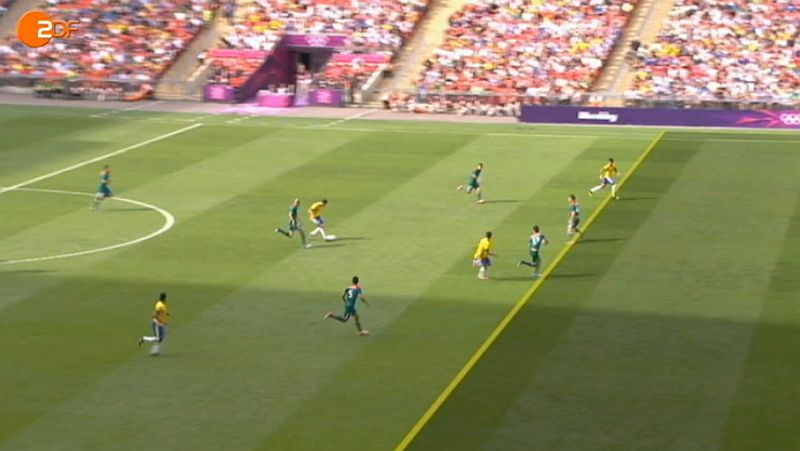
\includegraphics[width=0.9\textwidth]{graphics/augmented-reality/abseits}
		\caption{Augmented Reality (AR) bei Fu\ss{}ball-\"Ubertragungen{\cite{ar-soccer}}}
\end{figure} \\
\noindent In der Applikation 'Word Lens' wurde mithilfe von Augmented Reality eine Automatische Texterkennung, -\"ubersetzung und projektion realisiert. Mittels der Smartphone-Applikation kann der zu \"ubersetzende Text mit der integrierten Kamera erfasst und verarbeitet werden.

\begin{figure}[h!]
		\centering
		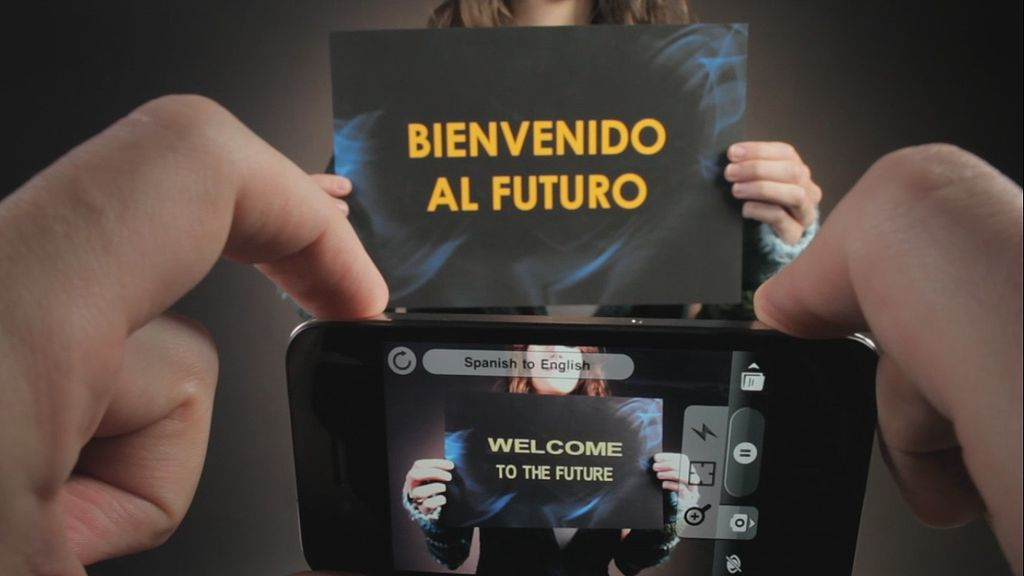
\includegraphics[width=0.7\textwidth]{graphics/augmented-reality/word-lens}
		\caption{Automatische Texterkennung, -\"ubersetzung und projektion in der Applikation Word Lens{\cite{auto-translate-ar}}}
\end{figure}
\noindent Die computergest\"utzte Erweiterung der Realit\"atswahrnehmung kann alle menschlichen Sinnesmodalit\"aten ansprechen und wird in industriellen Anwendungen, bei der Navigation, Geologie, Simulation, Architektur als auch in der Werbung und in vielen weiteren Bereichen verwendet.
\begin{figure}[h!]
		\centering
		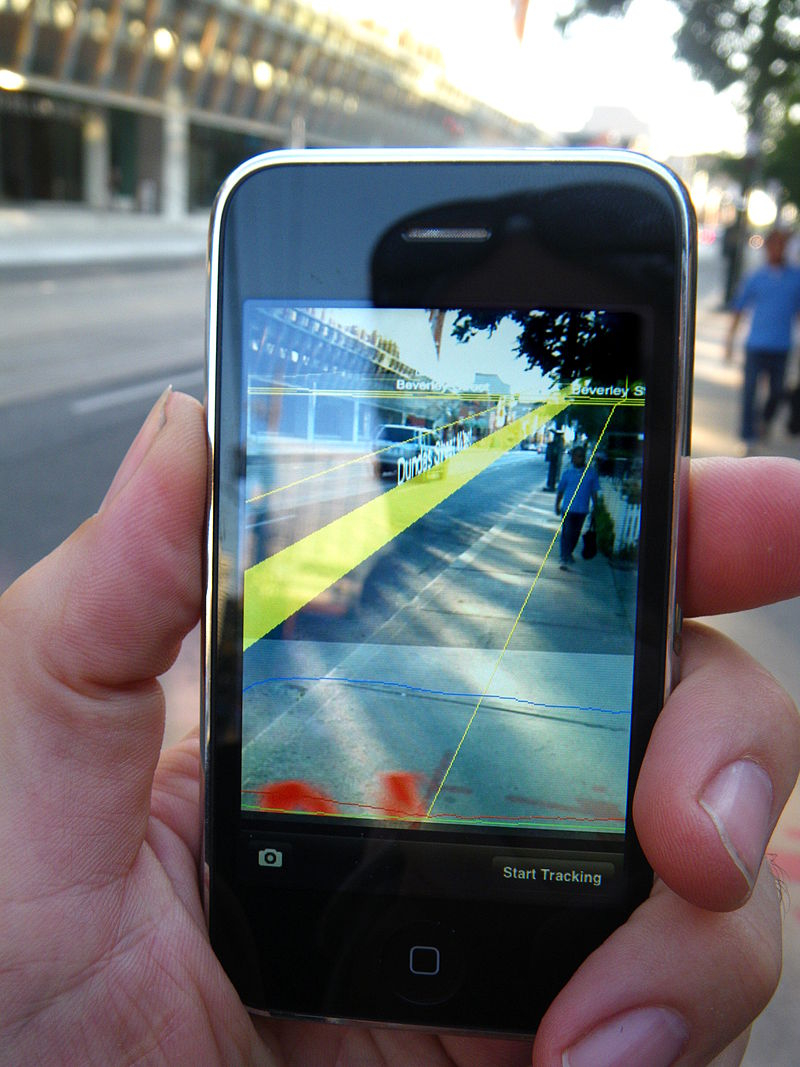
\includegraphics[width=0.4\textwidth]{graphics/augmented-reality/navigation}
		\caption{Navigationshinweis auf dem Smartphone mittels Augmented Reality{\cite{navi-ar}}}
\end{figure}
\begin{figure}[h!]
		\centering
		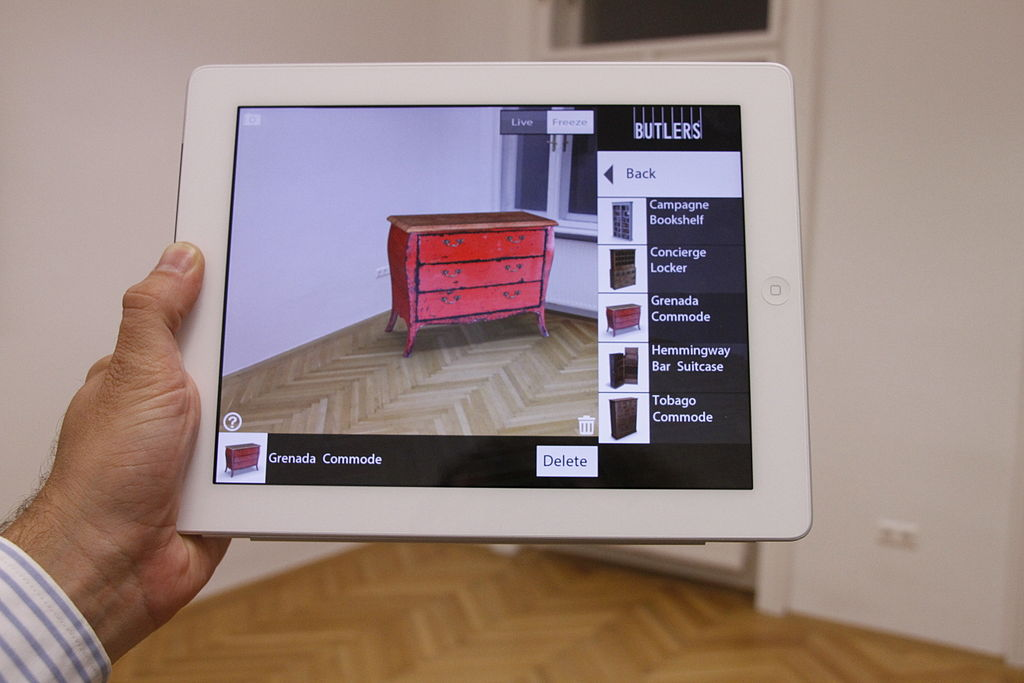
\includegraphics[width=0.7\textwidth]{graphics/augmented-reality/moebel}
		\caption{M\"obel als virtuelle Projektion{\cite{moebel-ar}}}
\end{figure} \\ \\

\newpage
\subsection{Implementierung Augmented Reality}
Die Implementierung der erweiterten Realit\"atswahrnehmung im Projekt 00SIRIS soll der intuitiven Steuerung zu Gute kommen. W\"ahrend sich das Team der Informationstechnologie um die software-technischen Aspekte gek\"ummert hat, war das Team der Maschinenbau f\"ur die Entwicklung der 3D-Modelle des Roboterarms zust\"andig. \\ \\
Diese wurden uns f\"ur das Einbauen der Augmented Reality zur Verf\"ugung gestellt. Das wesentliche Ziel war es, eine Objekterkennungsmethodik in unsere Android-Applikation zu integrieren. Die Aufgabe galt der Erschaffung eines Linienmodells, das f\"ur die Tracking-Algorithmen des von uns verwendeten Metaio-Software Development Kits notwendig war. Aus diesem galt es ein sogenanntes 'TubeModel' zu erstellen, das \"uber das erkannte Objekt gelegt wird, um die erfolgreiche Erkennung zu visualisieren.
\begin{figure}[h!]
		\centering
		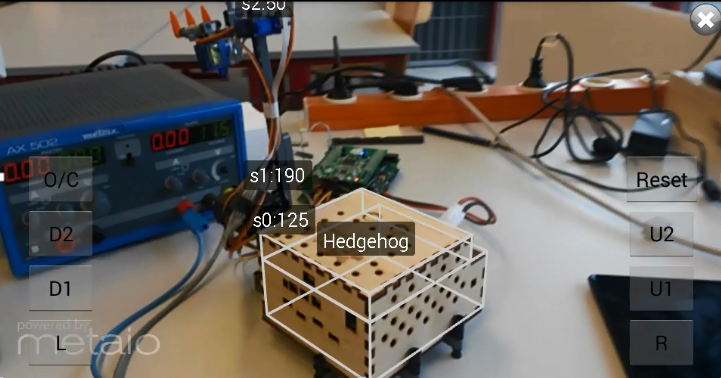
\includegraphics[width=0.7\textwidth]{graphics/augmented-reality/aug-andrej}
		\caption{Implementation der Augmented Reality beim Hedgehog Controller}
		\label{fig:hedgehog-controller-andrej}
\end{figure} \\
PRIA-Mitarbeiter Andrej Gall hat die Augmented Reality bereits bei dem Hedgehog Controller implementiert, die als Stütze für die Objekterkennung für 00SIRIS galt. Wie in der Abbildung 4.23 zu sehen ist, handelt es sich bei dem zu erkennenden Objekt um ein h\"olzernes Hedgehoggeh\"ause. \\ \\ 
\noindent Sobald das Objekt erkannt wurde und das TubeModel (ein wei\ss{}es Linienmodell) seinen rechtm\"a\ss{}igen Platz eingenommen hat, sollen die jeweiligen Werte der Hardwarekomponenten (Servomotoren, u.a. Sensoren) relativ zum Objekt angezeigt werden und deren Position, im Falle der \"Anderung des Blickwinkels \"andern. \\ \\

\newpage
\begin{figure}[h!]
		\centering
		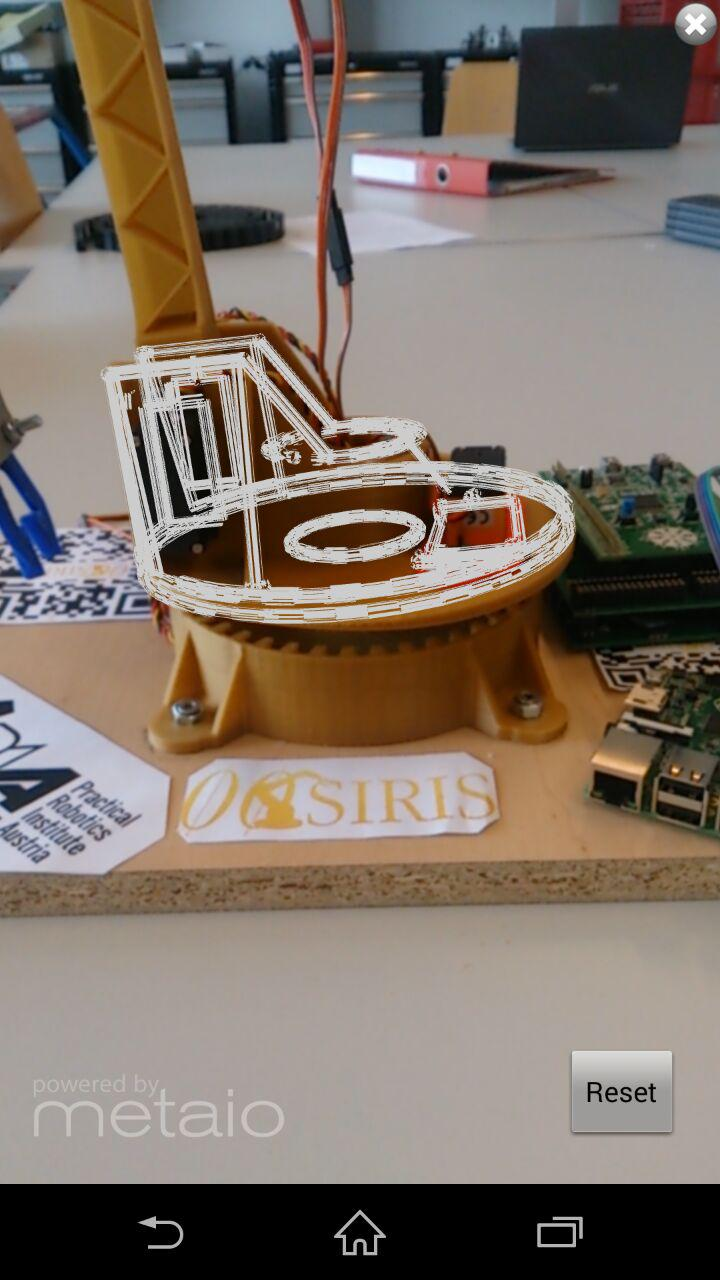
\includegraphics[width=0.4\textwidth]{graphics/augmented-reality/ar-osiris1}
		\caption{Implementation der Objekterkennung im Projekt 00SIRIS}
\end{figure}
Bei dem Projekt 00SIRIS erwies sich die Implementierung der Augmented Reality als schwierig, da es sich um eine wesentlich komplexere Form, als die des Hedgehogeh\"auses handelte. \\ \\
\noindent Aufgrund eines mangelnden Zeitbudgets wurde die Objekterkennung nicht in die eigentliche Steuerungsapplikation integriert und das Anzeigen der jeweiligen Werte der Hardwarekomponenten nicht vollst\"andig realisiert.


\newpage
\subsection{Sensoren an autonomen Robotern}
Der Einsatz von Industrierobotern in unserem allt\"aglichen Leben steigt stetig. Jede Aufgabe, die von einem Menschen gehandhabt wird, kann von einem Roboter mit h\"oherer Akkuratheit, mit weniger Zeitaufwand und mit einer wesentlichen geringeren Fehlerwahrscheinlichkeit gel\"ost werden.\\ 
Das Heben von gro\ss{}en Gewichten, als auch das pr\"azise Schwei\ss{}en von Schwei\ss{}n\"ahten kann somit durchgef\"uhrt werden. Weitere Robotersysteme, die in der Zukunft f\"ur den Menschen eine gro\ss{}e Rolle spielen werden, sind die autonomen Roboter. \\ \\
\textit{'Ein autonomer mobiler Roboter ist eine Maschine, die sich in einer nat\"urlichen Umgebung aus eigener Kraft und ohne Hilfestellung von au\ss{}en bewegen und dabei ein ihr gestelltes Ziel erreichen kann. [...] Dabei erkennt sie die Umwelt, sofern dies notwendig ist, \"uber eigene Sensoren.'} (P. Hoppen){\cite{robot-sensors}}\\ \\
Um diese Selbstst\"andigkeit, \"uber die ein Roboter dieser Form verf\"ugt, gew\"ahrleisten zu k\"onnen, sind wichtige Komponenten notwendig. Diese werden als Sensoren und Aktoren bezeichnet.

\paragraph{Sensoren}
In diesem Kapitel nehmen werden ausf\"uhrlichst jene Sensoren unter die Lupe genommen, die f\"ur die Entwicklung von 00SIRIS notwendig waren. \\\\
Prinzipiell werden Sensoren und Aktoren in extern und intern eingeteilt. Interne Sensoren finden Verwendung in der \"Uberwachung des inneren Zustandes eines Roboters, hingegen sind externe Sensoren f\"ur das Sammeln von Informationen \"uber die Roboterumgebung zust\"andig. Man kann Sensoren sozusagen als Sinnesorgane eines Roboters bezeichnen.\\ \\
Andere Klassifizierungen sind z.B. in aktive und passive Sensoren unterteilt.
\newpage
\begin{figure}[h!]
		\centering
		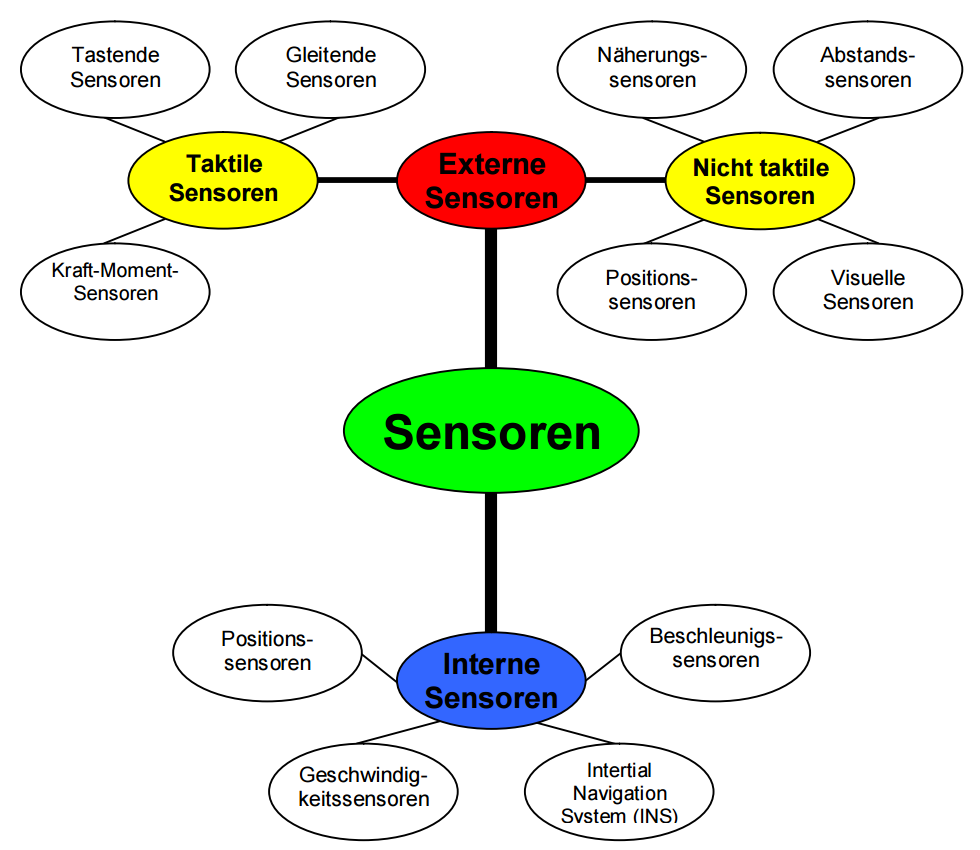
\includegraphics[width=0.9\textwidth]{graphics/sensors/klassifizierung}
		\caption{Klassifikation von Sensoren in der Robotik {\cite{robot-sensors}}}
\end{figure}
\noindent Taktile Sensoren finden Einsatz im Bereich des Robotergreifers und dienen zur Positionsbestimmung, Objekterkennung oder zur Ermittlung von Oberfl\"achenbeschaffenheit. Im Wesentlichen sind Taktile Sensoren f\"ur die Verteilung der Kraft des Greifers zust\"andig, sodass ein Objekt sicher gehalten werden kann und nicht besch\"adigt wird. Tastende, gleitende, als auch Kraft-Moment-Sensoren z\"ahlen zur Gruppe der Taktilen Sensoren und finden heutzutage im Bereich der Industrieroboter weitgehend Einsatz. \\ \\
Bei nicht taktilen Sensoren handelt es sich um jene Sensoren, die kapazitiver, induktiver, optischer, magnetischer oder auch akustischer Herkunft sind.{\cite{taktil-nicht-taktil}} \"Au\ss{}erst essentiell f\"ur die Sicherheit der Menschen, die mit Robotern hantieren m\"ussen, sind die N\"aherungssensoren, auf die im Kapitel Sicherheitssensorik n\"aher eingegangen wird.
\newpage
\begin{figure}[h!]
		\centering
		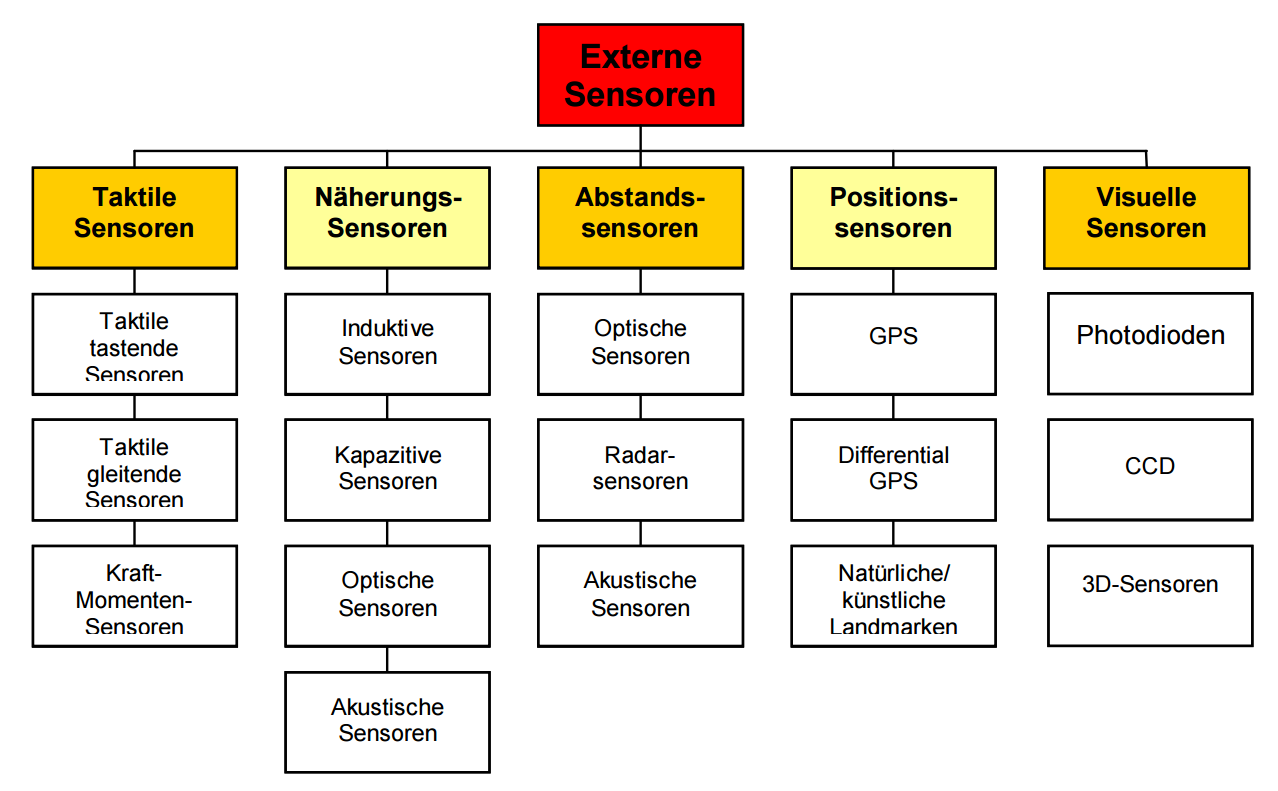
\includegraphics[width=1.0\textwidth]{graphics/sensors/externe-sensoren}
		\caption{\"Ubersicht 'Externe Sensoren'{\cite{robot-sensors}}}
\end{figure}
\noindent Unter 'Externen Sensoren' versteht man jene Sensoren, die Informationen \"uber die Umgebung des Roboters sammeln (Entfernung, Position, Hindernisse, Bilder in der Umgebung, etc).
Im Grundlegenden unterscheidet man zwischen Taktil- , N\"aherungs-, Abstands-, Positions- und
Visuellen Sensoren. \\ \\
Im Gegensatz zu den Taktilen Sensoren spezifizieren sich N\"aherungssensoren auf die Ortung von Objekten, um jeglichen Schaden, der durch das Ber\"uhren des Sensors verursacht wird, zu verhindern. Diese Art des Sensors findet in jenem Bereich Einsatz, in dem die Lebensdauer h\"ochste Priorit\"at hat. \\ \\
Der wohl bekannteste N\"aherungssensor ist die sogenannte Lichtschranke, dessen Funktionsweise und Aufbau ausf\"uhrlichst im Kapitel Sicherheitssensorik behandelt wird. \\ \\
Relevant f\"ur die Entwicklung des Prototypen waren die internen Positionssensoren sowie die
externen Abstandssensoren.
\newpage
\paragraph{Abstandssensoren}
Abstandssensoren fungieren mittels einer Entfernungsmessung zwischen dem Sensor und einem
Gegenstand. Der Einbau dieser kommt der Kollisionsvermeidung zu Gute und hilft dem Roboter sich
in seiner Umgebung orientieren zu k\"onnen. Im Wesentlichen wird zwischen optischen und
akustischen Abstandssensoren unterschieden. \\ \\
Der optische Abstandssensor erzeugt eine elektromagnetische Welle im nicht sichtbaren Bereich, die
mittels Triangulation zur Erkennung von r\"aumlichen Objekten dient. \\ \\
Durch die Projektion eines Laserstrahls auf einen entfernten Gegenstand wird das Licht des Strahls
reflektiert und an einen angebrachten Detektor (z.B. eine Kamera) weitergeleitet. Man erh\"alt den
Abstand zwischen Sender und Empf\"anger und die Entfernung zum Objekt kann mit der angegebenen
Triangulationsbeziehung berechnet werden. \\
\begin{figure}[h!]
		\centering
		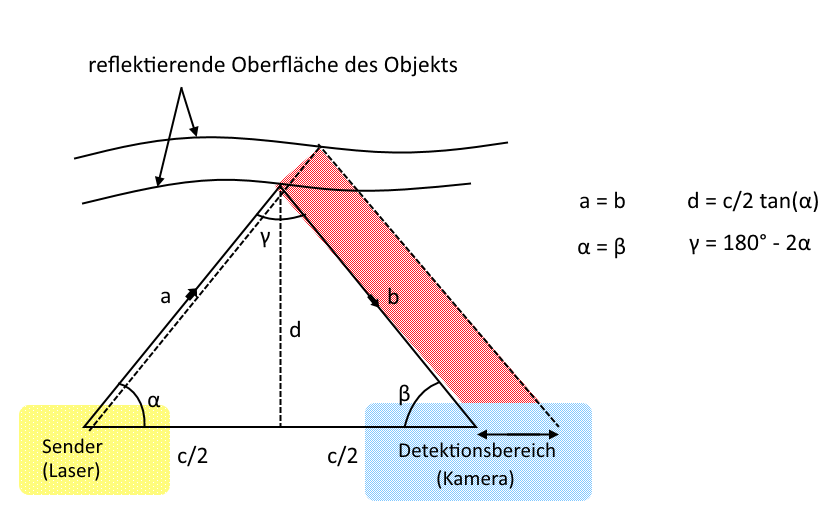
\includegraphics[width=1.0\textwidth]{graphics/sensors/triangulation-selfmade}
		\caption{Eine Illustration der Objektentfernungsmessung 'Triangulation'{\cite{robot-sensors}}}
\end{figure} 

\newpage
\begin{figure}[h!]
		\centering
		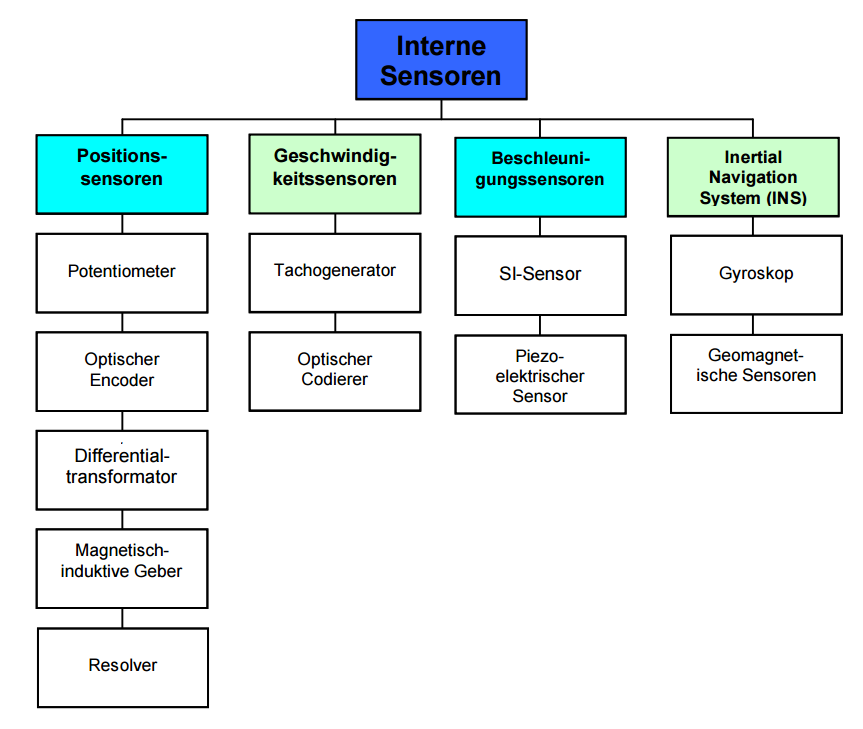
\includegraphics[width=0.9\textwidth]{graphics/sensors/interne-sensoren}
		\caption{\"Ubersicht 'Interne Sensoren'{\cite{robot-sensors}}}
\end{figure} 
\noindent Unter 'Internen Sensoren' versteht man jene Sensoren, die f\"ur die \"Uberwachung des inneren Zustands des Roboters zust\"andig sind. Zum Beispiel die Position, die Geschwindigkeit und die
Orientierung. \\ \\
Man kategorisiert diese in Positions-, Geschwindigkeits- und Beschleunigungssensoren sowie dem Inertial Navigation System (INS). \\ \\
Wie der Name schon sagt, liefert der Positionssensor Informationen \"uber die Position des Roboters.
Die einzelnen Positionen des Gelenkes und die jeweiligen Winkel der Achsen des Roboters k\"onnen
somit berechnet und weiterverarbeitet werden. \\ \\
Zu meist verwendeten Positionssensoren in der Robotik z\"ahlen: Potentiometer, Codierer,
Differentialtransformatoren, magnetisch-induktive Geber, Resolver, etc. \\ \\
Besonders interessant f\"ur die Entwicklung des Prototypen von 00SIRIS war der Einsatz von
Potentiometern.
\newpage
\paragraph{Potentiometer}
Bei einem Potentiometer handelt es sich um einen einstellbaren Spannungsteiler, der f\"ur die
Winkelmessung des Knickarmroboters verwendet worden ist. Dies ist insofern wichtig, da Grenzen
definiert werden k\"onnen um jeglichen Bewegungen, die den Roboterarm besch\"adigen w\"urden, zu
verhindern. \\
\begin{figure}[h!]
		\centering
		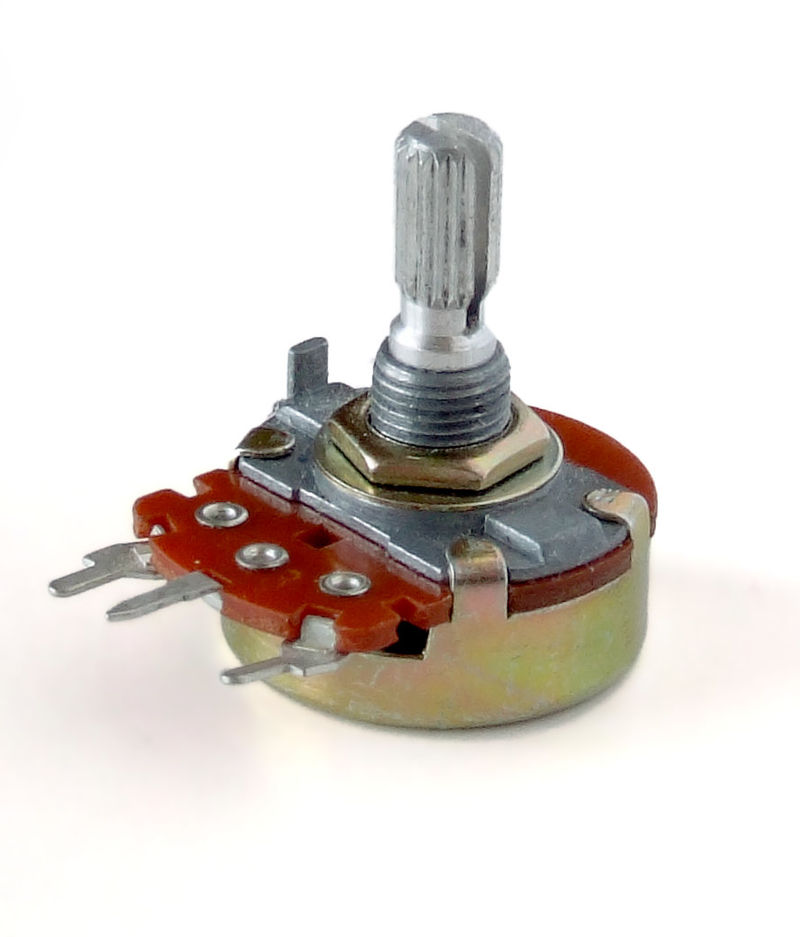
\includegraphics[width=0.5\textwidth]{graphics/sensors/potentiometer}
\end{figure} 
\begin{figure}[h!]
		\centering
		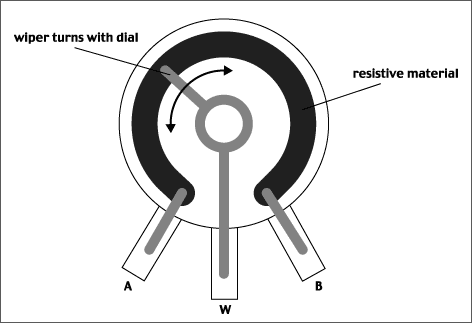
\includegraphics[width=0.5\textwidth]{graphics/sensors/potentiometer-inside}
\end{figure} 

\newpage
\section{Sicherheitssensorik}
Um das sichere Agieren mit Industrierobotern gew\"ahrleisten zu k\"osnnen, m\"ussen wesentliche Aspekte der Sicherheit beachtet werden.\cite{robot-sensors}
\paragraph{Optischer N\"aherungssensor}
Der Sensor, der im Bereich der Sicherheitssensorik am meisten Einsatz findet, ist der Optische N\"aherungssensor, oder auch als 'Lichtschranke' bekannt. \\ \\
Dieser arbeitet nach dem Schranken- und Reflexionsprinzip um eine gro\ss{}e Reichweite belegen zu k\"onnen. Die wesentlichen Bestandteile sind ein Lichtsender und ein Lichtempf\"anger. Von dem Lichtsender ausgehend wird ein Lichtstrahl an den Empf\"anger geschickt. Eine Unterbrechung dieses Strahls f\"uhrt zu einer Benachrichtigung des Systems, sodass diese dementsprechend handeln kann.\\ \\
\begin{figure}[h!]
		\centering
		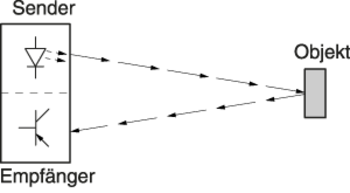
\includegraphics[width=0.4\textwidth]{graphics/sensors/optischer-naeherungssensor}
		\caption{Funktionsweise eines optischen N\"aherungssensors \cite{opt-sensor}}
\end{figure} \\
\noindent Ein weiterer Ansatz war die softwareunabh\"angige Implementierung eines Notausschalters, um jegliche Bewegungen der Servomotoren auf Knopfdruck zu stoppen. \\ \\
\begin{figure}[h!]
		\centering
		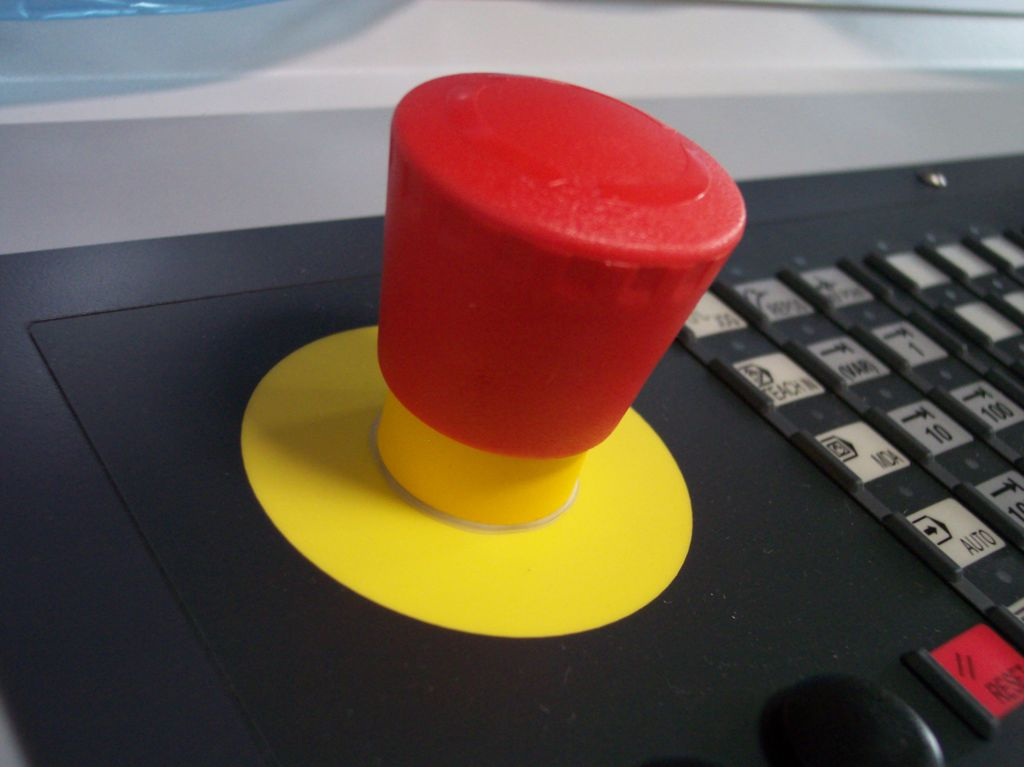
\includegraphics[width=0.3\textwidth]{graphics/sensors/notaus}
		\caption{Abbildung eines Notausschalters\cite{notaus-schalter}}
\end{figure}
\newpage
Im Alltag wird eine Lichtschranke zum Beispiel f\"ur das sichere Schlie\ss{}en der U-Bahnt\"uren eingesetzt.
\begin{figure}[h!]
		\centering
		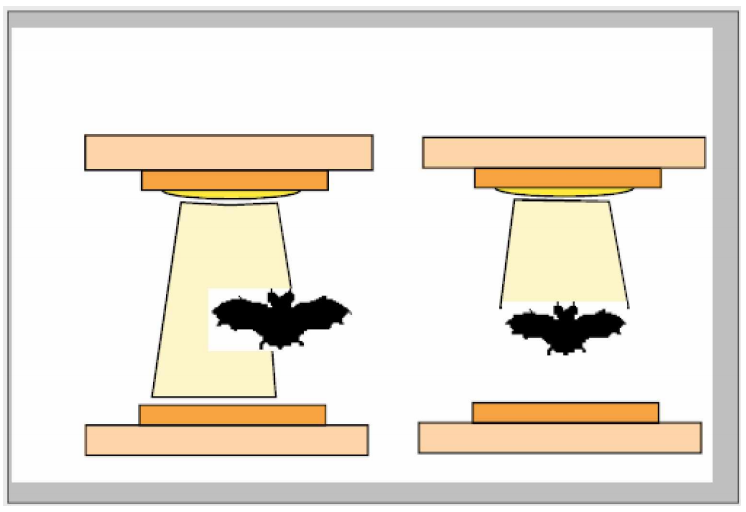
\includegraphics[width=0.8\textwidth]{graphics/sensors/lichtschranke}
		\caption{Abbildung einer Lichtschranke\cite{robot-sensors}}
\end{figure} \\
\noindent Die Lichtschranke findet bei so ziemlich allen industriellen Angelegenheiten Einsatz und erweist sich als \"au\ss{}erst n\"utzlich.
\begin{figure}[h!]
		\centering
		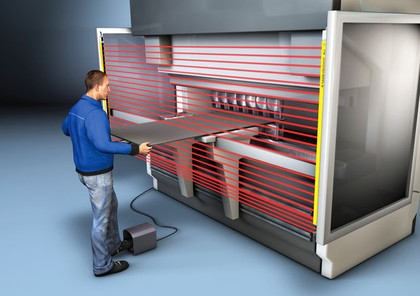
\includegraphics[width=0.8\textwidth]{graphics/sensors/lichtschranke-person}
		\caption{Eine Lichtschranke im Einsatz der Industrie\cite{lichtschranke-praxis}}
\end{figure}
\newpage
\paragraph{Kapazitiver N\"aherungssensor}
Mit einem kapazitiven N\"aherungsschalter wird eine ber\"uhrungsfreie \"Uberpr\"ufung auf eine Ann\"aherung eines leitenden oder nicht leitenden Gegenstandes erm\"oglicht.\\\\

Der Sensor an sich besteht aus einem Oszillator, einer Sensorelektrode und einem RS-Schwingkreis. Mithilfe des Schwingkreises wird ein elektrisches Feld erzeugt. Wenn sich nun ein Gegenstand der Elektrode n\"ahern sollte, kommt es zu einer \"Anderung der Kapazit\"at und der Oszillator f\"angt an zu schwingen. Auf diese Art und Weise werden sich n\"ahernde Objekte erfasst.\\\\

Die wohl vorteilhafteste Eigenschaft des kapazitiven N\"aherungssensors ist die Einsatzf\"ahigkeit in gef\"ahrlichen Umgebungen, da er in gro\ss{}en Abst\"anden reagiert.
\begin{figure}[h!]
		\centering
		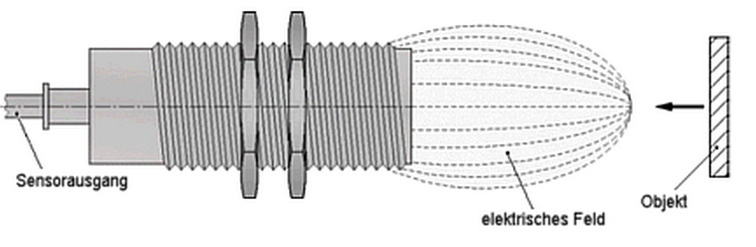
\includegraphics[width=0.9\textwidth]{graphics/sensors/kapazitiv-sensor}
		\caption{Abbild eines kapazitiven Sensors\cite{kapazitiv-sensor}}
\end{figure}


\newpage
\newpage
\nocite{*}
\bibliographystyle{plain}
\bibliography{bibliography}{}

\end{document}
